\documentclass[a4paper,10pt]{article}

\usepackage{amsmath,amssymb, amsthm}
\usepackage{charter}
%\usepackage{calc}

\usepackage{fullpage}

\usepackage{multirow}
%\usepackage[cp1250]{inputenc}
%\usepackage[T1]{fontenc}
%\usepackage{calligra}
%\usepackage[slovak]{babel}
\usepackage{amsfonts}
\usepackage{layout}
\usepackage[dvips]{graphicx}
\usepackage{url}
\usepackage{color}
\usepackage{graphicx}
\usepackage{algorithmic}
\usepackage{algorithm}
\usepackage{verbatim}
\usepackage{epsfig}
\usepackage[colorlinks,
            linkcolor=red,
            anchorcolor=blue,
            citecolor=blue
            ]{hyperref}
\usepackage{xcolor}

\renewcommand{\algorithmicrequire}{\textbf{Input:}}
\renewcommand{\algorithmicensure}{\textbf{Output:}}

\newcommand{\hlight}[2]{\noindent\colorbox{#1}{%
    \parbox{\dimexpr\linewidth-1\fboxsep}% a box with line-breaks that's just wide enough
        {#2%
        }}}

\newcommand{\HRule}{\rule{\linewidth}{0.5mm}}
 \newcommand{\xtilde}{\tilde x}
 \newcommand{\vtilde}{\tilde v}
 \newcommand{\Embb}{\E}
 \newcommand{\xbar}{\bar x}
 \newcommand{\ie}{\textit{i.e.}}
 
\newcommand{\main}[1]{\footnotesize\textbf{#1}} 
\newcommand{\todo}[1]{{\color{red}#1}}
\newcommand\tagthis{\addtocounter{equation}{1}\tag{\theequation}}


\newcommand{\del}[1]{{\color{red}#1}}

\let\la=\langle
\let\ra=\rangle

\newcommand{\st}{\;:\;}
\newcommand{\ve}[2]{\langle #1 ,  #2 \rangle}

\newcommand{\eqdef}{\stackrel{\text{def}}{=}}

\newcommand{\ii}{{}^{(i)}}

\newcommand{\R}{\mathbb{R}}
\newcommand{\Prob}{\mathbf{Prob}}
\newcommand{\E}{\mathbb{E}}
\newcommand{\Q}{\mathbb{Q}}
\newcommand{\Z}{\mathbb{Z}}

\newcommand{\vc}[2]{#1^{(#2)}}
\newcommand{\nc}[2]{{\color{red}\|#1\|_{(#2)}}}
\newcommand{\ncs}[2]{\|#1\|^2_{(#2)}}
\newcommand{\ncc}[2]{{\color{red}\|#1\|^*_{(#2)}}}
\newcommand{\ls}[1]{{\color{red} \mathcal S(#1)}}
\newcommand{\Rw}[2]{\mathcal R_{#1}(#2)}
\newcommand{\Rws}[2]{\mathcal R^2_{#1}(#2)}
\newcommand{\m}[1]{~\mbox{#1}~}

\newcommand{\nbp}[2]{\|#1\|_{(#2)}}   % norm block primal
\newcommand{\nbd}[2]{\|#1\|_{(#2)}^*} % norm block dual

\newcommand{\lf}{\mathcal L}
\newcommand{\U}{U}
\newcommand{\N}{N}
\newcommand{\mc}[1]{\mathcal #1}

\newcommand{\mLi}{{\color{red}m^{(i)}}}
\newcommand{\gLi}{{\color{red}g^{(i)}}}
%\newcommand{\TLi}{{\color{red}T_L^{(i)}}}
\newcommand{\TLi}[1]{{\color{blue}T^{(#1)}}}

\newcommand{\Lip}{L}

\newcommand{\Rc}[1]{{\color{red}  \mathbf{RC}_{(#1)}}}
\newcommand{\NRCDM}{{\color{red}NRCDM}\  }
\newcommand{\nnz}[1]{{\color{red}\|#1\|_0}}
% sets
\DeclareMathOperator{\card}{card}       % cardinality of a set
\DeclareMathOperator{\diam}{diam}       % diameter of a set
\DeclareMathOperator{\MVEE}{MVEE}       % minim volume enclosing ellipsoid of a set
\DeclareMathOperator{\vol}{vol}         % volume of a set

\DeclareMathOperator{\prox}{prox}         

% statistical
\DeclareMathOperator{\Exp}{\mathbf{E}}           % expectation
\DeclareMathOperator{\Cov}{Cov}         % covariance
\DeclareMathOperator{\Var}{Var}         % variance
\DeclareMathOperator{\Corr}{Corr}       % correlation

% functions and operators
\DeclareMathOperator{\signum}{sign}     % signum/sign of a scalar
\DeclareMathOperator{\dom}{dom}         % domain
\DeclareMathOperator{\epi}{epi}         % epigraph
\DeclareMathOperator{\Ker}{null}        % nullspace/kernel
\DeclareMathOperator{\nullspace}{null}  % nullpsace
\DeclareMathOperator{\range}{range}     % range
\DeclareMathOperator{\Image}{Im}        % image
\DeclareMathOperator{\argmin}{argmin}        % argmin

% topology
\DeclareMathOperator{\interior}{int}    % interior
\DeclareMathOperator{\ri}{rint}         % relative interior
\DeclareMathOperator{\rint}{rint}       % relative interior
\DeclareMathOperator{\bdry}{bdry}       % boundary
\DeclareMathOperator{\cl}{cl}           % closure

% vectors, matrices
\DeclareMathOperator{\linspan}{span}
\DeclareMathOperator{\linspace}{linspace}
\DeclareMathOperator{\cone}{cone}

\DeclareMathOperator{\tr}{tr}           % trace
\DeclareMathOperator{\rank}{rank}       % rank
\DeclareMathOperator{\conv}{conv}       % convex hull
\DeclareMathOperator{\Diag}{Diag}       % Diag(v) = diagonal matrix with v_i on the diagonal
\DeclareMathOperator{\diag}{diag}       % diag(D) = the diagonal vector of matrix D

\DeclareMathOperator{\Arg}{Arg}         % Argument

%\renewcommand{\qedsymbol}{\ding{114}}


\newtheorem{assumption}{Assumption}
\newtheorem{lemma}{Lemma}
\newtheorem{algorithms}{Algorithm}
\newtheorem{theorem}{Theorem}
\newtheorem{proposition}{Proposition}
\newtheorem{example}{Example}
\newtheorem{remark}{Remark}

\theoremstyle{plain}

\newtheorem{prop}[theorem]{Proposition}
\newtheorem{cor}[theorem]{Corollary}
\newtheorem{lem}[theorem]{Lemma}
\newtheorem{claim}[theorem]{Claim}
%\newtheorem{remark}[theorem]{Remark}

\theoremstyle{definition}

\newtheorem{exercise}[theorem]{Exercise}

\newtheorem{rem}[theorem]{Remark}
\newtheorem{que}[theorem]{Question}
\newtheorem{definition}[theorem]{Definition}

 
\title{Individual Contribution on his Project}
\author{Chenxin Ma, Xi He}
 
\begin{document}
\maketitle
 
We have a happy teamwork on this project. Because of the weak background we had on integer programming and programming on Python before this semester, each task we did in this project was from tremendous reading and thinking, each function we implemented was from many times revising and debugging. We met many difficulties, but luckily, we solved a majority of them. Every discussion was effective and encourages us to go further.  Both of us tried our best on this final project.   

~\\
\centerline{\textbf{Contribution from Chenxin Ma}}

In terms of implementation, I was responsible for implementing the first step in pre-processing, primal phase II procedure, dual phase II procedure, branch and bound algorithm. Typically, I wrote the following files: pre-processing.py, prime\_phase\_II.py, dual\_Phase\_II.py, Branching.py and a part in main.py. 

In terms of numerical experiment, I was responsible for those experiments on binary knapsack instances. Those instances are from the the author of the paper we studied,Prof. Goycoolea. 

In terms of writing report, I was responsible for describe algorithms I implemented and the experiments I made. 

The above things are mainly my contribution. However, a lot of them were finished after discussions and cooperation with Xi. I could not finish these tasks without teamwork. 

~\\
\centerline{\textbf{Contribution from Xi He}}
 
In this project, I implemented the pre-processing procedure pro.py which simplify the original problem, prime\_phase\_I.py, and domination.py. 

Besides, I make contribution in testing the algorithm and debug our implementation. In the numerical experiment part, I created the program that compared our implementation and the pulp with various of instants in a convenient way. I also generate random instants and recorded numerical results. 

In the report, I finished the description of those algorithms that Iimplemented, and analysis of numerical results. 

My mainly contribution is stated above. Throughout all this project, I discussed with Chenxin about the correct understanding of the paper and algorithm, and in order to implement our program correctly, efficiently and robustly, we debug and test each other's implementation. It's a cherish experience to work with Chenxin as a team and finished our project.

We use git to track and finish the whole project step by step, you may find the time-line about each work we did in this git repository.

\url{https://bitbucket.org/Xi_He/ip_proj/commits/all}

Also, I made a screenshot of our work for this project in the following two pages.
\begin{figure}[H]
\begin{center}
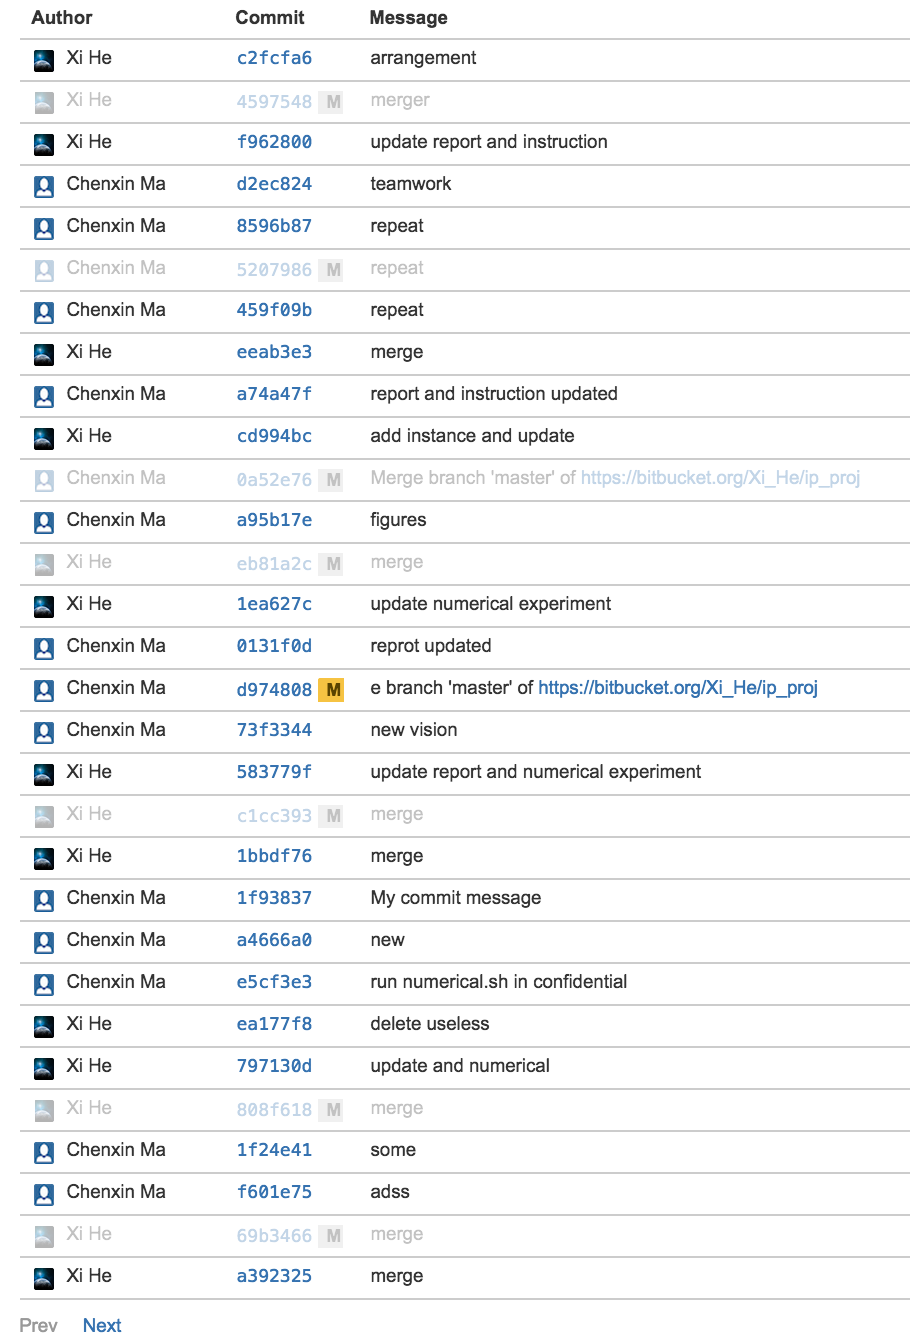
\includegraphics[scale=0.8]{git_1}
\end{center}
\end{figure}

\begin{figure}[H]
\begin{center}
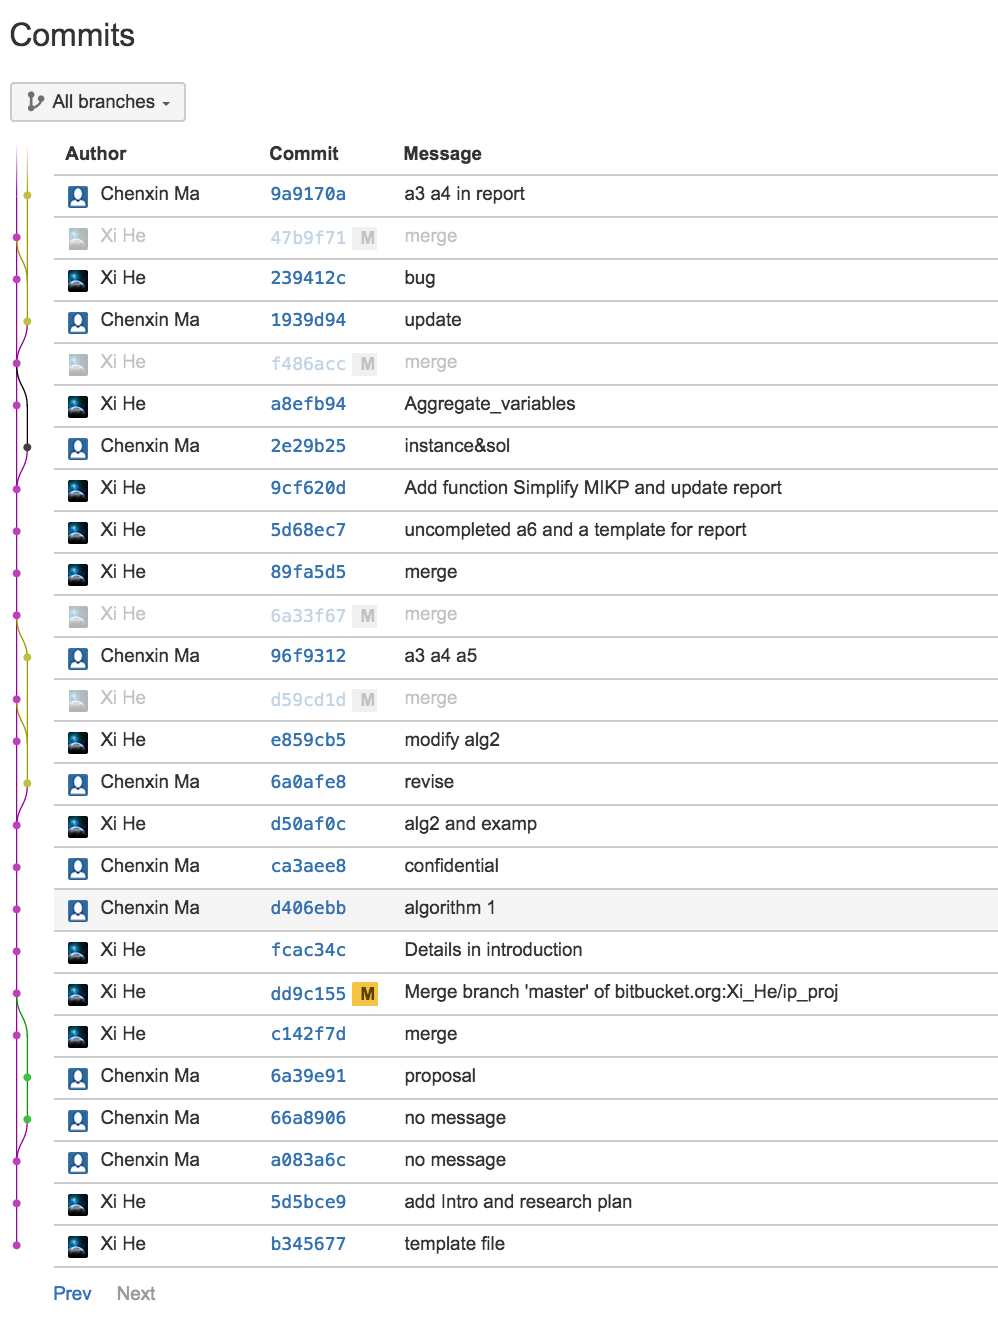
\includegraphics[scale=0.8]{git_2}
\end{center}
\end{figure}
\end{document}
